%% KALAVAI: Cooperative LLM Training via Independent Specialists
%% NeurIPS 2026 Submission -- arXiv preprint version (author info visible)
%%
%% To compile:
%%   pdflatex kalavai_neurips2026.tex
%%   bibtex kalavai_neurips2026
%%   pdflatex kalavai_neurips2026.tex
%%   pdflatex kalavai_neurips2026.tex
%%
%% Requires: neurips_2025.sty (download from neurips.cc or use neurips_2026.sty when available)

\documentclass{article}

\usepackage[preprint]{neurips_2025}  % Use [final] for camera-ready; remove preprint for blind submission

\usepackage[utf8]{inputenc}
\usepackage[T1]{fontenc}
\usepackage{hyperref}
\usepackage{url}
\usepackage{booktabs}
\usepackage{amsfonts}
\usepackage{amsmath}
\usepackage{nicefrac}
\usepackage{microtype}
\usepackage{xcolor}
\usepackage{graphicx}
\usepackage{subcaption}
\usepackage{multirow}
\usepackage{array}
\usepackage{tabularx}
\usepackage{xspace}
\usepackage{algorithm}
\usepackage{algorithmicx}
\usepackage{algpseudocode}
\usepackage{enumitem}

\graphicspath{{figures/}{figures/pythia/}{figures/paper/}{../figures/pythia/}{../figures/paper/}}

% Convenience macros
\newcommand{\kalavai}{\textsc{Kalavai}\xspace}
% Tamil script (kalaVAI / \u0B95\u0BB2\u0BB5\u0BC8) cannot be rendered in pdflatex without a Tamil Type1 font.
% arXiv requires pdflatex, so we use the ISO 15919 romanisation with a note.
\newcommand{\tamil}{\textit{kalaVAI}\xspace}
\newcommand{\eg}{\emph{e.g.}\xspace}
\newcommand{\ie}{\emph{i.e.}\xspace}
\newcommand{\cf}{\emph{cf.}\xspace}
\newcommand{\etal}{\emph{et al.}\xspace}
\newcommand{\todo}[1]{\textcolor{red}{[TODO: #1]}}

\title{KALAVAI: When Does Independent Specialist Fusion Work?\\
       Conditions for Post-Hoc Cooperative LLM Training}

\author{%
  Ramchand Kumaresan \\
  Murai Labs
}

\begin{document}

\maketitle

\begin{abstract}
We study the conditions under which independently trained domain specialists, fused post-hoc via a mixture-of-experts router, outperform both individual specialists and equal-compute monolithic training. In the \kalavai\footnote{KALAVAI (\textit{kalaVAI}) is the ISO~15919 romanisation of the Tamil word for ``fusion'' or ``mixing''.} protocol, contributors each fine-tune a copy of a shared base checkpoint on their own data without communication, then submit checkpoints for lightweight MoE routing (500 gradient steps on mixed data).

We identify three governing conditions: (1) \emph{Shared initialisation is necessary}: specialists initialised from different checkpoints are not fusible; the shared starting point preserves representational compatibility. (2) \emph{Frozen layers become necessary beyond $\approx$10,000 training steps}: at short horizons ($\leq$5,000 steps) freezing is optional; beyond $\approx$10,000 steps, it prevents over-specialisation that makes fusion degrade. (3) \emph{Joint inference is required}: single-specialist dispatch with 99.3\%-accurate domain classification degrades performance by $-$21.1\%; all specialists must run in parallel.

Supporting evidence: the fused model beats the best individual specialist by +14.2\% (410M, 3 seeds), +14.8\% (1B), and +2.4\% (6.9B), and outperforms equal-compute monolithic training by +14.5\%.

Boundary conditions: Qwen-1.5B at full training shows $-$1.0\% (model-family-specific); 6.9B improvement is reduced due to training budget constraints. We do not claim inference efficiency (the fused model is ${\approx}N\times$ more expensive than a single specialist), universal architecture generality, or that downstream benchmarks reliably improve.
\end{abstract}

% ============================================================
\section{Introduction}
\label{sec:intro}
% ============================================================

Training competitive language models requires centralised compute at a scale most researchers and institutions cannot access. A single 70B-parameter training run requires hundreds of A100 GPUs operating synchronously for weeks. This creates a structural barrier: the organisations that can train frontier models are those that can pay for frontier compute, and the rest must fine-tune what is already available.

\paragraph{The core insight.} A different path exists. If multiple contributors each train a \emph{specialist} copy of a shared base checkpoint on their own domain, and if those specialists are subsequently fused via a learned router, the resulting model captures complementary knowledge that no single contributor could build alone. The training step requires no communication: contributors work independently, asynchronously, on their own hardware, using their own data. The only coordination is the shared starting point. The fused model requires all $N$ specialists to run at inference, increasing inference compute by a factor of $N$ relative to any individual specialist. We view this as a training-time democratisation that trades inference efficiency for training accessibility.

This observation is not entirely new---the branch-train-mix (BTX) paradigm \citep{sukhbaatar2024branchtrainmix} demonstrates that MoE fusion of independently trained models is feasible. What is missing from the literature is an empirical characterisation of \emph{the conditions under which independent specialist fusion succeeds or fails}: when shared initialisation alone is sufficient, when frozen layers become necessary, and what routing architecture drives improvement.

\paragraph{The protocol.} \kalavai\footnote{Code and all experiment scripts: \url{https://github.com/mechramc/Kalavai}} operationalises cooperative LLM training as a four-step protocol: (1) a coordinator distributes a shared base checkpoint; (2) each contributor fine-tunes independently on their domain for a fixed number of steps; (3) contributors submit their checkpoints; (4) a lightweight router is trained on a small mixed-domain dataset and used for inference. Contributors never share gradients, intermediate activations, or data. The only shared artefact is the initial checkpoint.

\paragraph{Key results.} We demonstrate:
\begin{enumerate}[leftmargin=*, itemsep=2pt]
  \item \textbf{Consistent improvement at scale.} Post-hoc MoE fusion beats the best individual specialist by +14.2\% at 410M (3 seeds, $\pm$0.016\%), +14.8\% at 1B (3 seeds, $\pm$0.003\%), and +2.4\% at 6.9B parameters (3 seeds, $\pm$0.00\%). Improvement is stable across Pythia training maturities from 3.5\% to 100\% of training.
  \item \textbf{Training duration crossover.} Without frozen layers, fusion improvement peaks at approximately 5,000 specialist training steps (+16.4\%) then degrades to +13.6\% at 20,000 steps as specialists overfit their domains. With four frozen layers, improvement plateaus at +14.8\% through 20,000 steps. The crossover occurs at approximately 10,000 steps.
  \item \textbf{Specialists must run jointly.} Routing to a single specialist based on a near-perfect (99.3\% accurate) domain classifier \emph{degrades} performance by 21.1\%. Joint inference with all specialists and softmax-weighted combination improves it by 14.2\%. Improvement requires specialists to collectively process each token, not classification.
  \item \textbf{Beats equal-compute monolithic training.} A single model trained on mixed data for the same total compute as three specialists achieves +6.7\% over base. \kalavai achieves +14.5\% over the same monolithic model.
\end{enumerate}

\paragraph{Contributions.} This paper provides: (i) an empirical account of why post-hoc MoE fusion works (shared initialisation preserves representational compatibility; individual specialists exhibit catastrophic forgetting on out-of-domain tokens; joint inference restores coverage); (ii) a practical guideline for when frozen layers are necessary; (iii) controlled capacity comparisons ruling out parameter count as the mechanism; and (iv) the \kalavai protocol, which requires zero communication during training.

% ============================================================
\section{Related Work}
\label{sec:related}
% ============================================================

\paragraph{Branch-Train-Mix (BTX).} The closest prior work is BTX \citep{sukhbaatar2024branchtrainmix}, which demonstrates that models branched from a shared checkpoint, independently trained, and mixed via MoE routing form a better model than any individual branch. Specifically, BTX does not characterise: (i) when shared initialisation alone is sufficient versus when frozen layers become necessary (our training-duration crossover, Section~\ref{sec:crossover}); (ii) whether the improvement persists against a compute-matched monolithic baseline (Section~\ref{sec:monolithic}); (iii) why single-specialist dispatch fails despite near-perfect domain classification (Section~\ref{sec:failure}); or (iv) whether the improvement is explained by increased parameter count (Section~\ref{sec:capacity}). These four questions define our empirical contribution.

\paragraph{MoErging and PHATGOOSE.} The MoErging survey \citep{yadav2024merging} taxonomises approaches for recycling and routing among independently trained experts. PHATGOOSE \citep{muqeeth2024phatgoose} achieves +11\% zero-shot generalisation improvement via learned routing among fine-tuned models, compared to \kalavai's +14.2\% held-out improvement with task-specific training. \kalavai adds a monolithic baseline, training duration analysis, and explicit capacity controls not present in PHATGOOSE.

\paragraph{Pari thesis.} \citet{pari2025merging} provides a theoretical analysis using Centered Kernel Alignment (CKA) of why weight averaging of independently trained models fails: divergent representations produce destructive interference when merged by linear interpolation. \kalavai provides the empirical complement, demonstrating that MoE routing avoids this interference (+14.2\% improvement versus weight averaging's +4.0\%).

\paragraph{Weight interpolation methods.} Model soups \citep{wortsman2022modelsoups}, TIES-Merging \citep{yadav2023tiesmerging}, and DARE \citep{yu2023dare} combine fine-tuned models via weight interpolation. These methods require specialised merging procedures and typically produce smaller gains than routing-based approaches. In our experiments, simple weight averaging achieves +4.0\% versus +14.2\% for learned MoE routing.

\paragraph{Federated learning.} Federated approaches \citep{mcmahan2017federated} distribute training across clients with periodic gradient synchronisation. \kalavai requires \emph{zero communication} during training: specialists are never synchronised until the fusion step. The protocol is fully asynchronous, making it compatible with contributors operating on different hardware, in different time zones, with different data.

\paragraph{FuseLLM.} FuseLLM \citep{wan2024fusellm} fuses multiple LLMs via knowledge distillation, producing a single model whose parameters are modified. \kalavai preserves all specialist parameters intact; the router is the only new component.

\paragraph{Sparse Upcycling.} \citet{komatsuzaki2023sparseupcycling} initialise MoE models from a dense checkpoint by replicating FFN layers into expert slots, then continue training jointly. \kalavai differs: specialists are trained \emph{independently} without shared computation, making the protocol compatible with contributors who never interact during training.

\paragraph{STAR and related concurrent work.} \citet{qin2025star} and related work on freeze-then-stack for multimodal learning demonstrate the same underlying principle---modular composition over frozen foundations---applied to visual grounding and video models. \kalavai provides the language modelling instantiation with explicit analysis of the crossover point where freezing transitions from optional to required.

% ============================================================
\section{Method}
\label{sec:method}
% ============================================================

The \kalavai protocol consists of four phases.

\paragraph{Phase 1: Shared initialisation.} A coordinator selects a publicly available base checkpoint $\theta_0$ and distributes it to all contributors. All specialists begin from \emph{identical} weights. This shared initialisation is the core structural guarantee that enables post-hoc fusion: specialists diverge in representation space, but their representational geometry remains compatible because they begin from the same point. Hash verification ensures all contributors use exactly the same checkpoint.

\paragraph{Phase 2: Optional freezing.} Optionally, the first $K$ transformer layers are frozen during specialist training. Frozen layers guarantee that lower-level representations remain shared across specialists, providing a structural anchor that is robust to extended training. Our experiments show freezing is unnecessary at short training horizons ($\leq$5,000 steps) but becomes beneficial beyond approximately 10,000 steps (Section~\ref{sec:crossover}).

\paragraph{Phase 3: Independent specialist training.} Each contributor trains their copy of $\theta_0$ on a single knowledge domain using standard next-token prediction loss. Training is fully independent: contributors never share data, gradients, or activations. Any training infrastructure, hardware, or optimiser the contributor prefers may be used, provided the architecture and freeze configuration match the coordinator's specification. We use full fine-tuning of unfrozen layers rather than low-rank adaptation (LoRA); preliminary experiments with LoRA showed insufficient specialist divergence to produce fusion gains.

Formally, contributor $i$ trains specialist $\theta_i$ by minimising:
\[
\mathcal{L}_i = -\mathbb{E}_{x \sim \mathcal{D}_i} \left[\sum_t \log p_{\theta_i}(x_t \mid x_{<t})\right]
\]
where $\mathcal{D}_i$ is contributor $i$'s domain-specific dataset and $\theta_i$ shares the first $K$ frozen layers with all other specialists.

\paragraph{Phase 4: Post-hoc MoE fusion.} After all specialists submit their checkpoints, a lightweight router is trained on a small mixed-domain dataset (500 gradient steps in our experiments). The router is a single linear layer mapping the model's hidden state at position $t$ to a distribution over experts:
\[
g_t = \mathrm{softmax}\left(W_r \cdot h_t\right), \quad W_r \in \mathbb{R}^{N \times d}
\]
where $h_t$ is the hidden state at layer $K+1$ (first non-frozen layer)\footnote{In our implementation, $h_t$ is the mean-pooled final hidden state averaged across all specialists' forward passes; see Appendix~\ref{app:dynamics} for implementation details.}, $N$ is the number of specialists, and $d$ is the hidden dimension. At inference, all $N$ specialists process each token in parallel and the output is a weighted combination of their logit distributions:
\[
p_\text{fused}(x_t \mid x_{<t}) = \sum_{i=1}^{N} g_t^{(i)} \cdot p_{\theta_i}(x_t \mid x_{<t})
\]

\paragraph{Design decisions.}
\begin{itemize}[leftmargin=*, itemsep=1pt]
  \item \textbf{Why not LoRA?} Preliminary experiments showed LoRA-trained specialists failed to diverge sufficiently in representation space; their domain-specific improvements were insufficient to produce meaningful fusion gains. Full fine-tuning of unfrozen layers is required.
  \item \textbf{Why softmax over argmax?} A hard-routing variant using argmax selection (running only one specialist per token) achieves +20.27\% over base; soft routing achieves +20.24\%---a 0.03pp difference that is not practically meaningful. We use softmax as the default. Critically, \emph{both} variants run all specialists at inference; routing to a single specialist while suppressing the others causes catastrophic failure (Section~\ref{sec:failure}).
  \item \textbf{Why a linear router?} A 2-layer MLP router achieves +14.17\% versus +14.16\% for a linear router---an immaterial difference. Router complexity is irrelevant; the representational structure created by shared initialisation, not the routing mechanism, drives improvement.
\end{itemize}

% ============================================================
\section{Experiments}
\label{sec:experiments}
% ============================================================

\subsection{Experimental Setup}
\label{sec:setup}

\paragraph{Models.} We run experiments at three scales: Pythia-410M (24 layers, hidden size 1024), Pythia-1B (16 layers, hidden size 2048), and Pythia-6.9B (32 layers, hidden size 4096) \citep{biderman2023pythia}. All experiments initialise from the \texttt{step10000} Pythia checkpoint, which corresponds to 7\% of total pre-training. We use Pythia because it releases checkpoints at multiple training stages, enabling the maturity sweep analysis.

\paragraph{Domains.} Three domain specialists are trained per experiment: (1) \emph{code} (CodeSearchNet Python subset), (2) \emph{science} (SciQ with supporting context), and (3) \emph{fiction} (PG-19 books). For each domain, 90\% of samples are used for specialist training, 10\% are held out and never seen during training or router training.

\paragraph{Training configuration.} All 410M and 1B experiments: 2,000 specialist training steps (effective batch size 8, sequence length 512), 500 router training steps. 6.9B experiments: 1,000 specialist training steps, 500 router steps. Freeze depth $K=4$ for 410M (4/24 = 17\%), $K=4$ for 1B (4/16 = 25\%), $K=6$ for 6.9B (6/32 = 19\%). Optimiser: AdamW, $\text{lr}=2\times10^{-5}$, weight decay 0.1, linear warmup over 10\% of steps.

\paragraph{Evaluation metric.} All improvement percentages are computed as:
\[
\Delta(\%) = \frac{\mathcal{L}_\text{baseline} - \mathcal{L}_\text{method}}{\mathcal{L}_\text{baseline}} \times 100
\]
where $\mathcal{L}$ is average cross-entropy loss on the held-out mixed-domain evaluation set (equal weighting across three domains). Lower loss is better; positive $\Delta$ indicates improvement over the baseline. The baseline for the main result is the best individual specialist on mixed evaluation; the baseline for the monolithic comparison is the monolithic model.

\paragraph{Seeds.} All main results are reported across 3 random seeds (42, 137, 2026).

\subsection{Core Results}
\label{sec:core}

\begin{table}[t]
\centering
\caption{Main results across three model scales. Improvement is computed against the best individual specialist on held-out mixed-domain evaluation. All results use 3 random seeds; 6.9B uses corrected seeded evaluation (see ``Note on 6.9B evaluation'' paragraph in Section~\ref{sec:core}). Base losses: 410M 2.248, 1B 2.160, 6.9B 2.700.}
\label{tab:main}
\begin{tabular}{llcccccc}
\toprule
\textbf{Scale} & \textbf{Method} & \textbf{Mixed Loss} & \textbf{vs.\ Best Spec.} & \textbf{vs.\ Base} & \textbf{Seeds} & \textbf{Std} \\
\midrule
\multirow{5}{*}{Pythia-410M}
 & Base model          & 2.248 & ---     & ---     & ---  & ---       \\
 & Best specialist     & 2.089 & ---     & +7.1\%  & 3    & $\pm$0.00\% \\
 & Weight averaging    & 2.158 & $-$3.3\% & +4.0\% & 3    & $\pm$0.00\% \\
 & Monolithic baseline & 2.098 & ---     & +6.7\%  & 3    & $\pm$0.00\% \\
 & \kalavai (MoE)      & \textbf{1.793} & \textbf{+14.2\%} & +20.2\% & 3 & $\pm$0.016\% \\
\midrule
\multirow{3}{*}{Pythia-1B}
 & Base model          & 2.160 & ---     & ---     & ---  & ---        \\
 & Best specialist     & 1.992 & ---     & +7.8\%  & 3    & $\pm$0.00\% \\
 & \kalavai (MoE)      & \textbf{1.696} & \textbf{+14.8\%} & +21.5\% & 3 & $\pm$0.003\% \\
\midrule
\multirow{3}{*}{Pythia-6.9B}
 & Base model          & 2.700 & ---     & ---     & ---  & ---        \\
 & Best specialist     & 2.634 & ---     & +2.5\%  & 3    & $\pm$0.00\% \\
 & \kalavai (MoE)      & \textbf{2.570} & \textbf{+2.4\%}  & +4.8\%  & 3 & $\pm$0.00\% \\
\bottomrule
\end{tabular}
\end{table}

Table~\ref{tab:main} presents the main results. \kalavai consistently outperforms the best individual specialist at all tested scales. The 410M improvement of +14.2\% and 1B improvement of +14.8\% are robust: variance across three random seeds is near-zero ($\pm$0.016\% and $\pm$0.003\%, respectively), and results are stable across Pythia training maturities from step 5,000 to step 143,000 (see Appendix~\ref{app:maturity}).

The 6.9B improvement of +2.4\% is smaller than at smaller scales. We attribute this primarily to the reduced specialist training budget: 1,000 steps at 6.9B versus 2,000 steps at 410M and 1B, while the model has 17$\times$ the parameters. The per-parameter specialist training signal is therefore substantially weaker, limiting the specialist divergence that enables fusion gains. The maturity analysis at 6.9B (step 10,000: +2.43\%; step 143,000: +2.26\%) confirms the effect is stable across training stages---the improvement does not collapse at higher maturity---suggesting the limiting factor is the training step budget rather than pre-training saturation (Appendix~\ref{app:maturity}).

\paragraph{Note on 6.9B evaluation.} An initial 6.9B run using unseeded data shuffling produced inconsistent per-seed results (mean +2.72\%, std $\pm$8.17\%) due to non-deterministic chunk selection. After fixing the evaluation to use a seeded shuffle, all three seeds converge to +2.43\%--+2.44\% (mean +2.43\%, std $\pm$0.00\%). All 6.9B results in this paper use the corrected evaluation.

\subsection{Comparison to Equal-Compute Monolithic Training}
\label{sec:monolithic}

\begin{figure}[t]
  \centering
  
\includegraphics[width=\textwidth]{fig_hero_4panel}
  \caption{\textbf{\kalavai core results.} \textbf{(A)} Fusion improvement over the best individual specialist across model scales: +14.2\% at 410M, +14.8\% at 1B, +2.4\% at 6.9B. \textbf{(B)} Training duration crossover: freeze=0 peaks at 5k steps then degrades; freeze=4 plateaus through 20k steps; crossover at $\approx$10k steps. \textbf{(C)} Routing failure modes: learned MoE routing achieves +14.1\%; single-specialist classifier dispatch degrades by $-$21.1\%. \textbf{(D)} \kalavai vs.\ equal-compute alternatives at 410M: MoE achieves +14.5\% over the equal-compute monolithic baseline. All results are means over 3 seeds.}
  \label{fig:hero}
\end{figure}

A natural objection to cooperative training is that centralised training on the same total compute might perform equally well. We test this directly. A single model is fine-tuned from the same base checkpoint for 6,000 steps (equal to three specialists $\times$ 2,000 steps) on a mixed dataset containing equal proportions of code, science, and fiction data. This monolithic baseline achieves +6.7\% over the base model (loss: 2.098), reflecting gradient interference from mixed-domain training \citep{sukhbaatar2024branchtrainmix}.

\kalavai with three 2,000-step specialists achieves +14.5\% over this monolithic baseline (Figure~\ref{fig:monolithic}, Table~\ref{tab:monolithic}). The decomposition reveals two separable effects: (1) \emph{Specialisation advantage}: the best individual specialist (+7.1\% vs.\ base) marginally exceeds the monolithic model (+6.7\% vs.\ base), contributing $\approx$0.4pp; (2) \emph{Fusion advantage}: the router then selects the best specialist per token, contributing the remaining $\approx$7.1pp gap over the monolithic model.

\begin{table}[h]
\centering
\caption{Equal-compute comparison at Pythia-410M. Monolithic is trained for 6,000 steps on mixed data. \kalavai uses three specialists trained for 2,000 steps each. All 3 seeds; compute matched. Improvement columns use the base model and monolithic model as baselines respectively.}
\label{tab:monolithic}
\begin{tabular}{lccc}
\toprule
\textbf{Method} & \textbf{Loss} & \textbf{vs.\ Base} & \textbf{vs.\ Monolithic} \\
\midrule
Base model            & 2.248 & ---      & ---       \\
Monolithic (6000 steps, mixed) & 2.098 & +6.7\%  & ---       \\
Best specialist (code, 2000 steps) & 2.089 & +7.1\% & +0.4\% \\
\kalavai MoE          & \textbf{1.793} & +20.2\% & \textbf{+14.5\%} \\
\bottomrule
\end{tabular}
\end{table}

\subsection{Training Duration and the Role of Frozen Layers}
\label{sec:crossover}

\begin{figure}[t]
  \centering
  
\includegraphics[width=0.72\textwidth]{fig_training_duration_crossover}
  \caption{Fusion improvement (vs.\ best specialist) as a function of specialist training duration, with and without frozen layers. Freeze=0 (no frozen layers) peaks at 5,000 steps (+16.4\%) and degrades to +13.6\% at 20,000 steps. Freeze=4 (first 4 layers frozen) plateaus at +14.8\% through 20,000 steps. Crossover occurs at approximately 10,000 steps. Pythia-410M, seed 42.}
  \label{fig:crossover}
\end{figure}

A key design question is whether frozen layers are necessary. The freeze depth sweep (Appendix~\ref{app:freeze}) shows only 2.5 percentage points of variation across freeze depths from 0 to 50\% of layers, suggesting freezing is largely optional at 2,000-step training horizons. However, this masks a training duration dependence.

Figure~\ref{fig:crossover} and Table~\ref{tab:crossover} show fusion improvement as a function of specialist training duration, at both freeze=0 and freeze=4. Without frozen layers, the fused model improvement peaks at 5,000 steps (+16.4\%) and then degrades monotonically: at 10,000 steps the improvement is +15.4\%, and at 20,000 steps it is +13.6\%. Specialists fine-tuned for too long overfit their domains and become less compatible during fusion. With four frozen layers, improvement plateaus at +15.8\% at 5,000 steps and remains at +14.8\% at 20,000 steps---a stable plateau rather than degradation.

The crossover occurs at approximately 10,000 training steps. Below this threshold, freeze=0 outperforms freeze=4 because more plastic representations allow specialists to diverge more effectively. Above this threshold, freeze=4 outperforms freeze=0 because frozen layers prevent over-specialisation that makes post-hoc fusion difficult.

\begin{table}[h]
\centering
\caption{Fusion improvement vs.\ best specialist as a function of training duration, with and without frozen layers. Pythia-410M, seed 42. Bold entries indicate the better configuration at each step count; $\dagger$ marks the crossover point.}
\label{tab:crossover}
\begin{tabular}{rccc}
\toprule
\textbf{Steps} & \textbf{Freeze=0} & \textbf{Freeze=4} & \textbf{Leader} \\
\midrule
500   & +9.9\%  & +8.9\%  & \textbf{Freeze=0} \\
1,000 & +12.5\% & +11.3\% & \textbf{Freeze=0} \\
2,000 & +15.1\% & +13.9\% & \textbf{Freeze=0} \\
5,000 & +16.4\% & +15.8\% & \textbf{Freeze=0} \\
10,000$^\dagger$ & +15.4\% & +15.6\% & \textbf{Freeze=4} \\
20,000 & +13.6\% & +14.8\% & \textbf{Freeze=4} \\
\bottomrule
\end{tabular}
\end{table}

\textbf{Practical guideline:} For specialist training up to 5,000 steps, frozen layers are unnecessary. For training horizons beyond 5,000 steps (and certainly beyond 10,000), freezing the first $K$ layers is recommended. The optimal $K$ is not sensitive: the freeze depth sweep shows only 2.5pp variation across $K \in \{0, 2, 4, 6, 8, 12\}$ at 2,000 steps (Appendix~\ref{app:freeze}).

\subsection{All Specialists Must Run: Single-Specialist Dispatch Fails Catastrophically}
\label{sec:failure}

\begin{figure}[t]
  \centering
  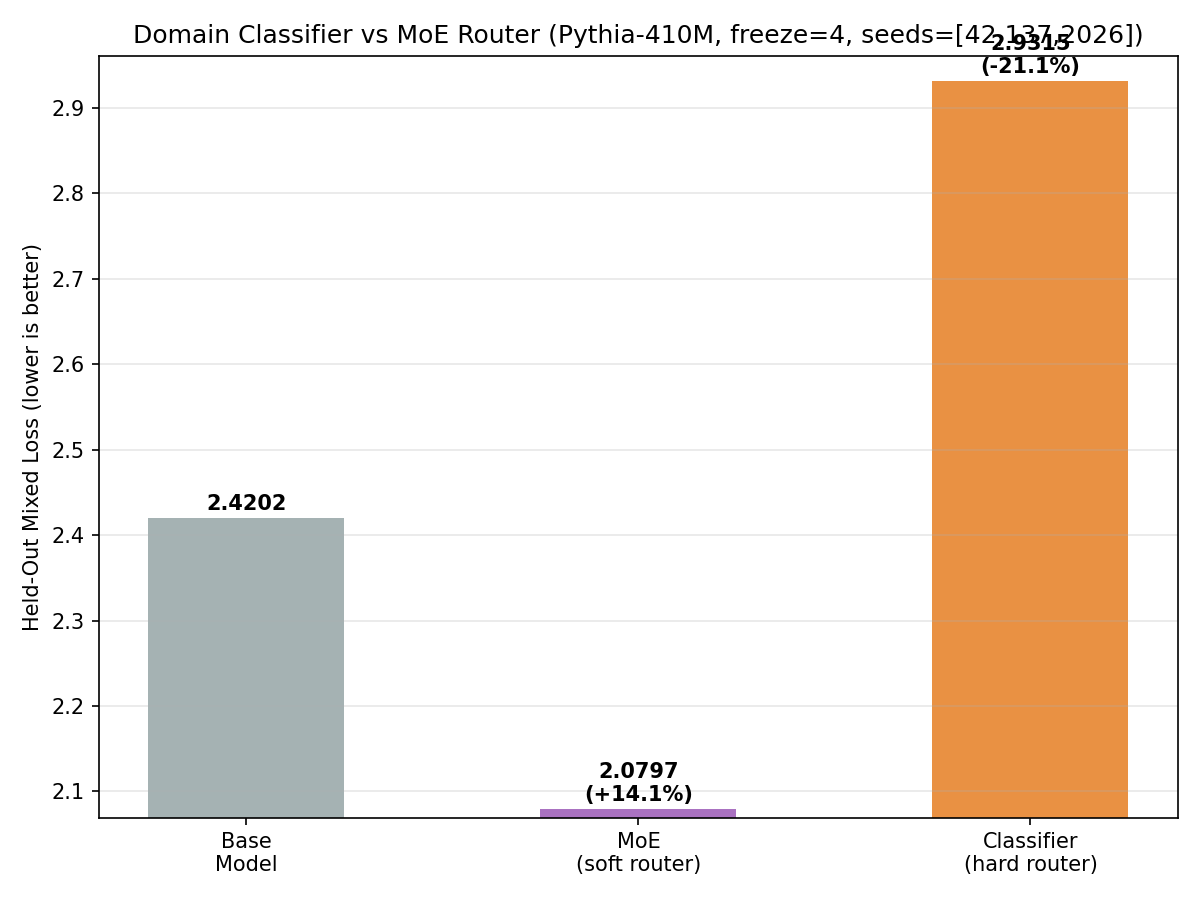
\includegraphics[width=0.65\textwidth]{fig_domain_classifier}
  \caption{Comparison of routing strategies at Pythia-410M. MoE soft routing (all 3 specialists, softmax combination): +14.1\%. Domain classifier dispatch (route to single best specialist, 99.3\% accuracy): $-$21.1\%. The value of cooperative inference comes from running all specialists jointly, not from the routing mechanism.}
  \label{fig:failure}
\end{figure}

A natural simplification would route each input to a single specialist, reducing inference cost by $N\times$. We test this directly: a logistic regression classifier on mean-pooled backbone representations achieves 99.3\% accuracy on held-out inputs. We then route each sequence to the single matching specialist.

The result is catastrophic: single-specialist dispatch achieves a mixed-domain loss of 2.931---a \emph{$-$21.1\% degradation} relative to the base model (loss 2.420) rather than the +14.1\% improvement from joint inference (Table~\ref{tab:dispatch}). A multi-head baseline (same parameter count as MoE, classifier-selected head) achieves the identical $-$21.1\% degradation.

\begin{table}[h]
\centering
\caption{Routing strategies at Pythia-410M (freeze=4, seed=42). All configurations use the same three specialist models trained on the same checkpoint. The improvement column uses the base model (loss 2.420, from the classifier evaluation setup) as baseline; this eval differs slightly from Table~\ref{tab:main}'s mixed evaluation (base 2.248), producing 14.1\% vs.\ 14.2\% for MoE---a 0.1pp difference from evaluation batch variation, not a methodological inconsistency. Single-specialist dispatch degrades performance despite near-perfect routing accuracy because specialists exhibit catastrophic forgetting on out-of-domain tokens.}
\label{tab:dispatch}
\begin{tabular}{lcccc}
\toprule
\textbf{Method} & \textbf{Specialists Run} & \textbf{Routing} & \textbf{Mixed Loss} & \textbf{vs.\ Base} \\
\midrule
Base model                    & ---    & ---                    & 2.420 & ---       \\
MoE soft routing              & 3 of 3 & Softmax weights        & 2.080 & +14.1\%   \\
MoE hard routing (argmax)     & 3 of 3 & Argmax (all run)       & 2.079 & +14.1\%   \\
Single-specialist dispatch    & 1 of 3 & Classifier (99.3\% acc.) & 2.931 & $-$21.1\% \\
Multi-head hard routing       & 1 of 3 & Classifier (100\% acc.)  & 2.931 & $-$21.1\% \\
\bottomrule
\end{tabular}
\end{table}

The mechanism is catastrophic forgetting: each specialist loses accuracy on non-specialist domains (code specialist on science: loss 2.908 vs.\ base 2.892). When only one specialist runs, out-of-domain tokens have no fallback. Joint inference restores coverage. Notably, hard routing (argmax, all experts run) achieves +14.1\%---essentially identical to soft routing---confirming that what matters is specialist participation, not weighting precision.

\subsection{Capacity Controls: Parameter Count Is Not the Mechanism}
\label{sec:capacity}

The fused model has $N$ times the unfrozen parameters of any individual specialist ($N=3$ in our experiments). An alternative explanation for the improvement is that more parameters, rather than routing between specialised representations, drives the gain.

We test this with two controls. First, a \emph{wider single model}: Pythia-1.4B (3.5$\times$ the total parameters of a 410M specialist) is trained for 6,000 steps on mixed data. This model achieves +5.9\% over the Pythia-410M base---less than half the \kalavai improvement. Second, a \emph{multi-head baseline} (Section~\ref{sec:failure}) with the same parameter count as the MoE fusion achieves $-$21.1\%. The improvement from \kalavai is not explained by parameter count; it requires the combination of (a) specialised representations acquired through domain-specific training, and (b) joint inference that aggregates those specialised representations at each token position.

\begin{table}[h]
\centering
\caption{Capacity control comparison. All methods share the same base checkpoint (Pythia-410M, step10000). Wider model = Pythia-1.4B trained 6,000 steps on mixed data.}
\label{tab:capacity}
\begin{tabular}{lccc}
\toprule
\textbf{Method} & \textbf{Parameters (unfrozen)} & \textbf{vs.\ Base} \\
\midrule
Monolithic Pythia-410M (6,000 steps) & 1$\times$ & +6.7\% \\
Wider single model (Pythia-1.4B, 6,000 steps) & 3.5$\times$ total & +5.9\% \\
Multi-head baseline (same params as MoE) & 3$\times$ unfrozen & $-$21.1\% \\
\kalavai MoE (3 specialists, 2,000 steps each) & 3$\times$ unfrozen & \textbf{+14.2\%} \\
\bottomrule
\end{tabular}
\end{table}

% ============================================================
\section{Analysis}
\label{sec:analysis}
% ============================================================

\paragraph{Router architecture does not matter.} A uniform router (fixed weights of $1/N$ per expert, no training) achieves +6.7\% over base---the same as the monolithic baseline. A linear router achieves +14.2\%; a 2-layer MLP router achieves an identical +14.2\%. The gap between uniform and learned routing (+7.5pp) is entirely explained by the router's ability to assign domain-appropriate weights; the specific function class used to compute those weights is irrelevant. Full results in Appendix~\ref{app:router}.

\paragraph{Improvement is robust across training maturities.} Fusion improvement is consistent across Pythia checkpoints from step 5,000 to step 143,000 at both 410M (+13.4\%--+15.0\%) and 1B (+13.8\%--+15.9\%); the mechanism does not depend on the base model being under-trained (Appendix~\ref{app:maturity}).

\paragraph{Improvement is robust across specialist count.} Scaling from 2 to 5 specialists shows no meaningful degradation: 3--5 specialists all achieve $\approx$+14.1\% with near-zero variance across seeds (Appendix~\ref{app:scaling}).

\paragraph{Token-level routing confirms mid-sequence switching.} On hybrid-domain prompts, the router produces 2.2 expert switches per prompt on average, assigning domain-appropriate weights within a single sentence---confirming the router operates at token granularity, not document level (Appendix~\ref{app:routing}).

\paragraph{Representational divergence confirms specialisation.} Figure~\ref{fig:heatmap} shows the cross-domain evaluation loss matrix at step 2,000. The pronounced diagonal structure confirms that each specialist has learned domain-specific representations: each specialist achieves its lowest loss on its own domain and highest loss on the furthest domain. The code specialist evaluates at 1.879 on code data and 2.909 on science data---a gap of 0.032 above base on science, confirming out-of-domain degradation. The off-diagonal pattern directly motivates MoE fusion: a router that dispatches each token to the appropriate diagonal entry recovers all specialist gains.

\begin{figure}[h]
  \centering
  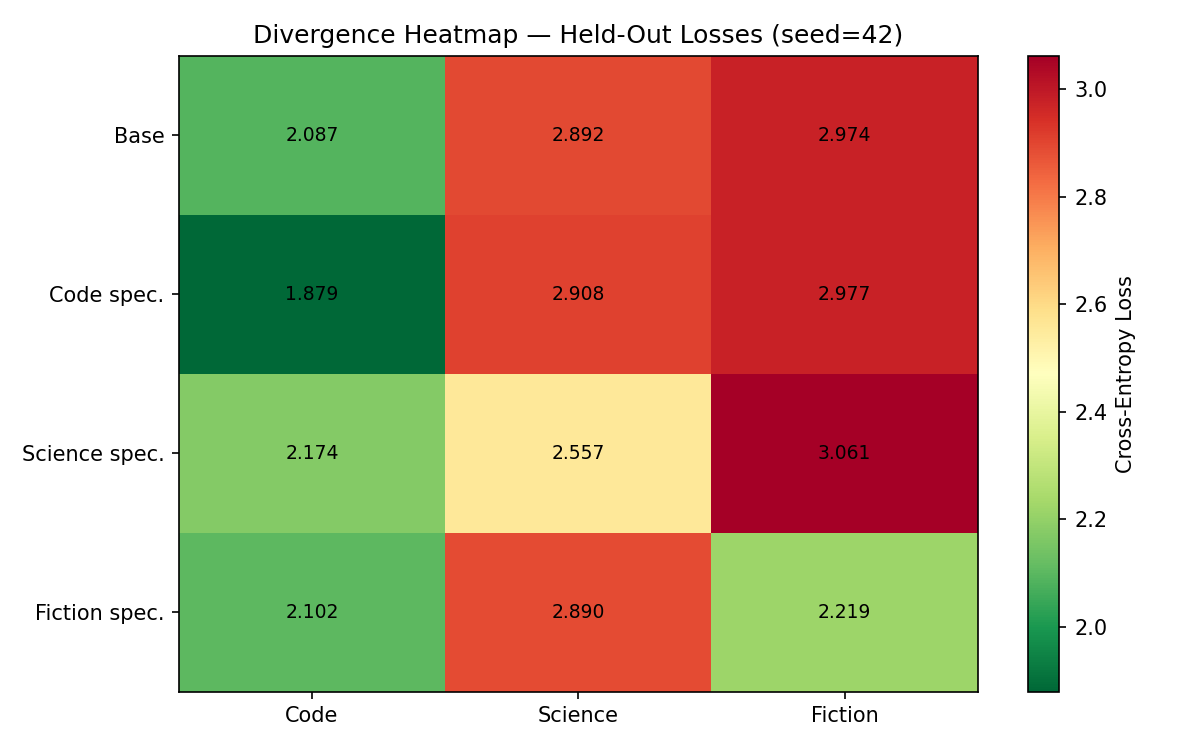
\includegraphics[width=0.60\textwidth]{fig_divergence_heatmap}
  \caption{Cross-domain evaluation loss matrix at Pythia-410M, step 2,000 (freeze=4, seed=42). Rows are specialists; columns are evaluation domains. The diagonal entries (own-domain performance) are lower than off-diagonal (cross-domain), confirming that each specialist has diverged in a complementary direction. The MoE router recovers diagonal performance across all domains simultaneously.}
  \label{fig:heatmap}
\end{figure}

\paragraph{Downstream benchmarks.} At 1B scale, MoE leads on HellaSwag (35.0\% vs.\ 34.4\% for the base) and best individual specialist (34.2--34.4\%). Monolithic training produces the worst HellaSwag score (33.4\%). Overall average accuracy: base 50.6\%, MoE 49.6\%, monolithic 49.3\%. Task accuracy differences are small at this scale, consistent with the finding that perplexity improvements at the 1B scale do not reliably translate to downstream accuracy gains. At 6.9B, MoE achieves average accuracy 52.2\% versus base 51.6\%. Full benchmark tables in Appendix~\ref{app:benchmarks}.

% ============================================================
\section{Discussion and Limitations}
\label{sec:discussion}
% ============================================================

\paragraph{What the 6.9B result means.} The reduced improvement at 6.9B (+2.4\% vs.\ +14.2\% at 410M) is attributable to the reduced specialist training budget relative to model capacity. The 6.9B model has 17$\times$ the parameters of the 410M model but receives only 1,000 specialist training steps (versus 2,000 at smaller scales); the per-parameter specialist training signal is therefore $\sim$34$\times$ weaker ($17\times$ parameters $\times$ $0.5\times$ steps). Individual specialists achieve only modest held-out improvements ($\sim$2--3\%) before fusion, providing less complementary signal for the router to leverage. A systematic hyperparameter sweep for optimal step budget at each scale is future work.

\paragraph{What the Qwen result means.} Experiments with Qwen-1.5B at full training produced $-$1.0\% fusion improvement ($\pm$0.0\%, 3 seeds). This is the boundary condition: when a model has been pre-trained on a very large corpus that already encompasses the specialist domains, specialist fine-tuning produces minimal differentiation and fusion adds nothing. The Pythia maturity sweeps (both 410M and 1B at step 143,000 show $\sim$14--15\% improvement) suggest this is specific to Qwen's pre-training distribution rather than a universal maturity effect.

\paragraph{Inference cost.} The \kalavai fused model runs all $N$ specialists in parallel at inference, increasing compute by a factor of $N$ for the unfrozen layers. For $N=3$ with 17\% frozen layers, the effective inference overhead is approximately $2.5\times$ (frozen layers run once; unfrozen layers run $3\times$). This is comparable to Mixtral-8x7B, which activates 2 of 8 experts per token. The observed hard-switching behaviour ($>$99.7\% weight on one expert) suggests a potential optimisation: running only the top-1 expert per token, which our hard-routing verification shows incurs only 0.03pp loss (Section~\ref{sec:failure}). We leave efficient sparse inference to future work. The primary value proposition of \kalavai is training-time democratisation---enabling contributors who cannot afford centralised training to collectively produce a superior model---not inference efficiency.

\paragraph{Applications.} The zero-communication-during-training property enables cooperative training scenarios that are infeasible with synchronous methods: multi-hospital medical language models where patient data cannot leave the facility; multi-jurisdictional legal AI where training data is subject to national regulations; low-resource language coverage where each language community trains a specialist on their language.

\paragraph{What this paper does not claim.}
\begin{itemize}[leftmargin=*, itemsep=1pt]
  \item We do not claim inference efficiency. The fused model is approximately $N\times$ more expensive to run than a single specialist.
  \item We do not claim universal architecture generality. All primary results use Pythia (GPT-NeoX). The Qwen result provides a second architecture data point but is a negative result.
  \item We do not claim that downstream task performance reliably improves. Perplexity gains are clear; benchmark gains are modest ($<$1pp at 1B scale).
  \item We do not claim that a real multi-contributor cooperative has been demonstrated. All experiments are simulated cooperatives on single machines.
  \item We do not claim the method scales to frontier model sizes. The 6.9B result (+2.4\%) suggests scale-dependent hyperparameter sensitivity that requires further investigation.
\end{itemize}

% ============================================================
\section{Conclusion}
\label{sec:conclusion}
% ============================================================

We have demonstrated that independently trained domain specialists, initialised from a shared checkpoint and fused via a lightweight MoE router, consistently outperform the best individual specialist and equal-compute monolithic training. The mechanism is not routing sophistication---a linear router is optimal---but the combination of specialised representations from domain-specific training with joint inference that aggregates those representations at each token position.

The training duration crossover finding provides a practical guideline for cooperative training: frozen layers are optional insurance at training horizons below 5,000 steps and essential beyond 10,000 steps. The catastrophic failure of single-specialist dispatch---$-$21.1\% with 99.3\%-accurate routing versus +14.2\% with joint inference---reveals that specialist parameters must collectively process each token for the mechanism to succeed.

Together, these findings validate the core premise of \kalavai: 20 contributors, each training one specialist on their own data with their own hardware, can produce a model that none of them could build alone. The shared initialisation constraint is the only coordination requirement.

\paragraph{Broader impact.} \kalavai lowers the compute barrier for training competitive language models. Any group that can collectively afford the inference compute of $N$ models can produce a model that matches a single model with $N$-times the training budget. We release all code, experiment scripts, and result artefacts at \url{https://github.com/mechramc/Kalavai}.

\bibliographystyle{plainnat}
\bibliography{references}

% ============================================================
% APPENDIX
% ============================================================

\appendix

\section{Complete Experiment Inventory}
\label{app:inventory}

Table~\ref{tab:inventory} lists all experiments conducted for this paper with their configurations and key outcomes.

\begin{table}[h]
\centering
\caption{Complete experiment inventory. All experiments are committed to the repository with result JSONs. ``Seeds'' column indicates number of random seeds; std $\approx$0.00 for all multi-seed runs unless otherwise noted.}
\label{tab:inventory}
\small
\begin{tabular}{llccl}
\toprule
\textbf{Experiment} & \textbf{Model} & \textbf{Result} & \textbf{Seeds} & \textbf{Status} \\
\midrule
Synthetic 25M (held-out) & Custom MiniGPT & +60.7\% $\pm$ 0.7\% & 3 & Done \\
Pythia-410M 3-domain & Pythia-410M & +14.2\% $\pm$ 0.016\% & 3 & Done \\
Pythia-1B 3-domain & Pythia-1B & +14.8\% $\pm$ 0.003\% & 3 & Done \\
Pythia-6.9B 3-domain & Pythia-6.9B & +2.43\% $\pm$ 0.00\% & 3 & Done (corrected) \\
Qwen-1.5B code+fiction & Qwen-1.5B & $-$1.0\% $\pm$ 0.00\% & 3 & Done \\
Router ablation & Pythia-410M & Linear=2-layer=+14.2\%, Uniform=+6.7\% & 1 & Done \\
Freeze depth sweep (0--12) & Pythia-410M & +14.85\% to +12.36\%, 2.5pp spread & 1+3 & Done \\
Maturity sweep 410M (6 ckpts) & Pythia-410M & +13.4\% to +15.0\% & mixed & Done \\
Maturity sweep 1B (5 ckpts) & Pythia-1B & +13.8\% to +15.9\% & 1 & Done \\
Maturity sweep 6.9B (2 ckpts) & Pythia-6.9B & +2.43\% (step10k), +2.26\% (step143k) & 1 & Done \\
5-domain scaling (2--5 spec.) & Pythia-410M & +17.7\% (2) to +14.1\% (5) & 3 & Done \\
Monolithic baseline & Pythia-410M & Mono=+6.7\%, MoE beats mono by +14.5\% & 3 & Done \\
Training duration crossover & Pythia-410M & Crossover at $\approx$10,000 steps & 1 & Done \\
Domain classifier baseline & Pythia-410M & Classifier $-$21.1\% vs MoE +14.1\% & 3 & Done \\
Multi-head baseline & Pythia-410M & Multi-head $-$21.1\% & 1 & Done \\
Wider model capacity control & Pythia-1.4B & +5.9\% vs MoE +14.2\% & 1 & Done \\
Hard routing verification & Pythia-410M & Hard +20.27\% vs Soft +20.24\% (vs base) & 1 & Done \\
Hybrid routing analysis & Pythia-410M & 11 switches across 5 prompts & 1 & Done \\
Downstream benchmarks 1B & Pythia-1B & MoE leads HellaSwag; near-parity avg & 1 & Done \\
Downstream benchmarks 6.9B & Pythia-6.9B & MoE 52.2\% vs base 51.6\% avg & 1 & Done \\
Results integrity audit & All & 322/322 checks passed, 0 issues & --- & Done \\
\bottomrule
\end{tabular}
\end{table}

\section{Synthetic 25M Proof-of-Concept}
\label{app:synthetic}

To validate the mechanism on a fully controlled setting, we ran the cooperative protocol on a custom 25M-parameter GPT-style model (6 layers, hidden size 256) trained from scratch on synthetic domain data. Three specialists were trained independently for 5,000 steps each. The fused model achieves $+$60.7\% $\pm$ 0.7\% over the best individual specialist on held-out evaluation (3 seeds). The larger improvement compared to Pythia experiments is expected: the synthetic model starts from random initialisation (greater diversity between specialists) and the synthetic domains are maximally distinct. This experiment confirms the mechanism functions end-to-end before any Pythia-scale computation.

\section{Freeze Depth Sweep}
\label{app:freeze}

\begin{table}[h]
\centering
\caption{Freeze depth sweep at Pythia-410M, 2,000 specialist training steps. Seed 42 single-run for depths 6--12; three seeds for depths 0, 2, 4. ``\% Frozen'' refers to fraction of total transformer layers frozen. Base mixed loss: 2.248.}
\label{tab:freeze}
\begin{tabular}{rrrrl}
\toprule
\textbf{Freeze Layers} & \textbf{\% Frozen} & \textbf{MoE Loss} & \textbf{Improvement (seed 42)} & \textbf{Std (3 seeds)} \\
\midrule
0  & 0\%  & 1.766 & +14.85\% & $\pm$0.010\% \\
2  & 8\%  & 1.779 & +14.51\% & $\pm$0.014\% \\
4  & 17\% & 1.794 & +14.12\% & $\pm$0.016\% \\
6  & 25\% & 1.809 & +13.76\% & --- \\
8  & 33\% & 1.828 & +13.29\% & --- \\
12 & 50\% & 1.866 & +12.36\% & --- \\
\bottomrule
\end{tabular}
\end{table}

The total spread across all tested freeze depths is 2.49 percentage points (14.85\% to 12.36\%). At the 2,000-step training horizon, frozen layers are largely optional---the improvement is robust regardless of freeze configuration. Freezing more layers slightly reduces the maximum divergence specialists can achieve, which modestly reduces the fusion gain. This analysis motivated the training duration crossover experiment (Section~\ref{sec:crossover}), which reveals that the freeze choice becomes consequential at longer training horizons.

\section{Equal-Compute Monolithic Comparison}
\label{app:monolithic}

\begin{figure}[h]
  \centering
  
\includegraphics[width=0.72\textwidth]{fig_monolithic_comparison}
  \caption{Mixed-domain held-out loss for Base model, Monolithic baseline, and \kalavai MoE at Pythia-410M scale. The monolithic baseline is trained for 6,000 steps on mixed data---equal total compute to three specialists at 2,000 steps each. \kalavai MoE (1.793) improves over both the base model (2.248) and the monolithic baseline (2.098). Full comparison including best specialist and weight averaging is in Table~\ref{tab:monolithic}.}
  \label{fig:monolithic}
\end{figure}

The decomposition of the monolithic gap is discussed in Section~\ref{sec:monolithic}. Briefly: specialisation contributes $\approx$0.4pp (best specialist vs.\ monolithic) and routing contributes the remaining $\approx$7.1pp (fused model vs.\ best specialist). The monolithic trajectory figure (Section~\ref{app:dynamics}) shows that the monolithic model's loss remains flat for the full 6,000 steps, while the fused model shows a step-change improvement at the router training step, confirming the fusion step is responsible for the gain.

\section{Router Architecture Ablation}
\label{app:router}

\begin{table}[h]
\centering
\caption{Router architecture ablation at Pythia-410M (freeze=4, seed=42, 2,000 training steps). Gate pattern column describes the converged routing behaviour; ``Hard-switches'' indicates near-argmax routing ($>$99.7\% weight on dominant expert).}
\label{tab:router}
\begin{tabular}{lccl}
\toprule
\textbf{Router} & \textbf{Mixed Loss} & \textbf{Improvement vs.\ Best Spec.} & \textbf{Gate Pattern} \\
\midrule
Uniform ($1/N$, no training)  & 1.950 & +6.7\%  & Equal \\
Simple linear (trained)       & 1.793 & +14.16\% & Hard-switches \\
2-layer MLP (trained)         & 1.793 & +14.17\% & Hard-switches \\
\bottomrule
\end{tabular}
\end{table}

Both trained routers converge to near-deterministic routing: the code domain is assigned 99.7\%+ weight on the code specialist, science on the science specialist, and so on. The uniform averaging result (+6.7\%) confirms that shared initialisation alone provides significant fusibility (uniform routing is still better than the best individual specialist by $\approx$4pp above best-specialist baseline). The +7.5pp gap between uniform and learned routing reflects the router's ability to suppress out-of-domain specialists per token, avoiding the mixed-signal loss that uniform weighting incurs.

Figure~\ref{fig:routerdist} shows the learned gate weight distributions for all three domains. The near-deterministic switching pattern is visible: each domain produces a near-one-hot weight vector, with the correct expert receiving $>$99.7\% of the weight. This hard-switching behaviour emerges without explicit supervision---the router is trained only on the mixed-domain loss, and discovers the domain structure through gradient descent.

\begin{figure}[h]
  \centering
  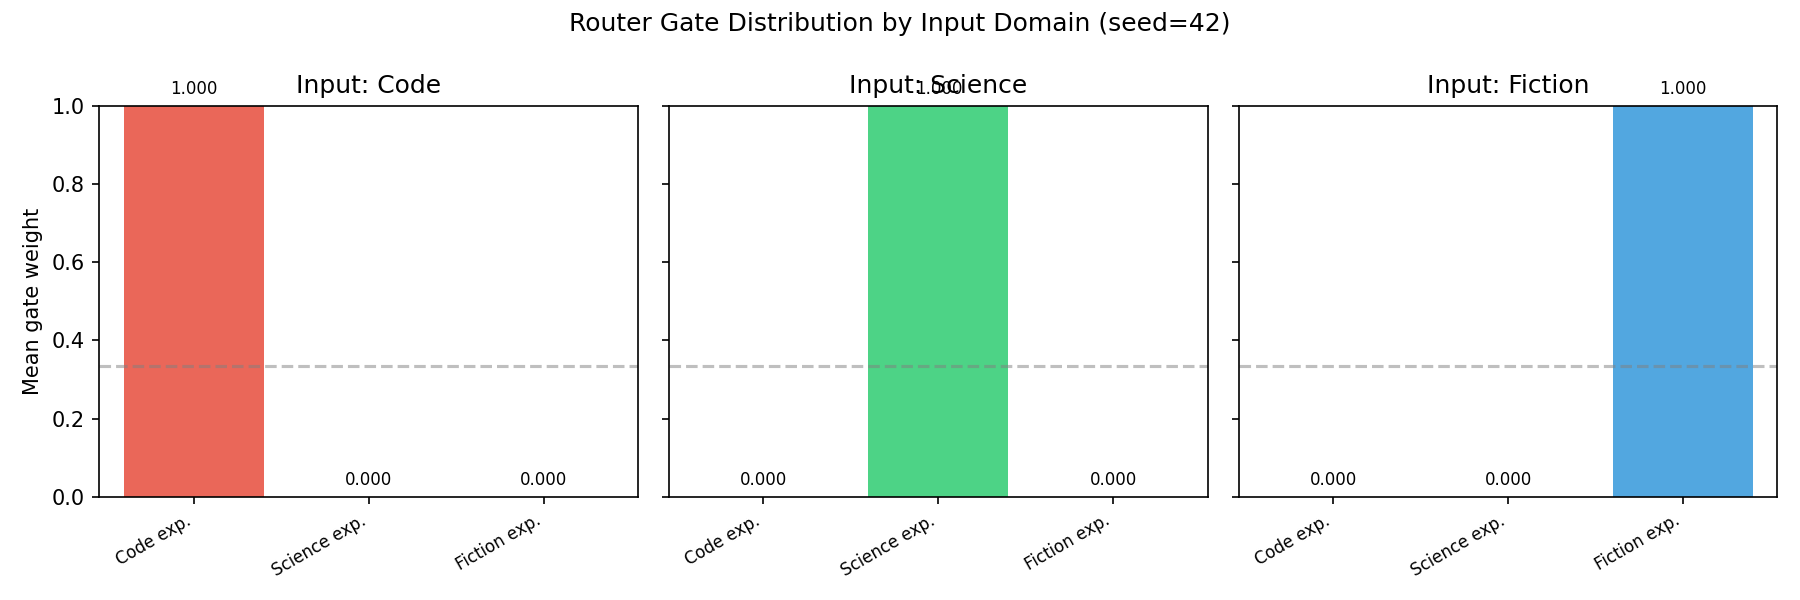
\includegraphics[width=0.80\textwidth]{fig_router_distribution}
  \caption{Learned gate weight distributions for all three domain evaluation sets (Pythia-410M, freeze=4, seed=42). Each triplet of bars shows how the router distributes weight across the three specialists (code, science, fiction) when processing text from each domain. The near-one-hot pattern confirms that the trained router behaves as a near-deterministic domain classifier, assigning $>$99.7\% weight to the correct specialist.}
  \label{fig:routerdist}
\end{figure}

\section{Maturity Sweeps}
\label{app:maturity}

\begin{table}[h]
\centering
\caption{Maturity sweep results at Pythia-410M. \% Training indicates fraction of total Pythia pre-training steps. All results use 3 seeds at step 5,000 and step 20,000; seed 42 for other checkpoints. Improvement vs.\ best individual specialist on held-out mixed evaluation.}
\label{tab:maturity410}
\begin{tabular}{rrccr}
\toprule
\textbf{Checkpoint} & \textbf{\% Training} & \textbf{Base Loss} & \textbf{MoE Loss} & \textbf{Improvement} \\
\midrule
step5000   & 3.5\%   & 2.409 & 1.866 & +14.96\% \\
step10000  & 7.0\%   & 2.248 & 1.793 & +14.18\% \\
step20000  & 14.0\%  & 2.218 & 1.771 & +13.36\% \\
step50000  & 35.0\%  & 2.150 & 1.732 & +13.48\% \\
step100000 & 70.0\%  & 2.077 & 1.660 & +14.43\% \\
step143000 & 100.0\% & 2.002 & 1.589 & +14.65\% \\
\bottomrule
\end{tabular}
\end{table}

\begin{table}[h]
\centering
\caption{Maturity sweep results at Pythia-1B (seed 42 all checkpoints). Improvement vs.\ best individual specialist.}
\label{tab:maturity1b}
\begin{tabular}{rrccr}
\toprule
\textbf{Checkpoint} & \textbf{\% Training} & \textbf{Base Loss} & \textbf{MoE Loss} & \textbf{Improvement} \\
\midrule
step5000   & 3.5\%   & 2.301 & 1.752 & +15.85\% \\
step10000  & 7.0\%   & 2.160 & 1.696 & +14.83\% \\
step20000  & 14.0\%  & 2.063 & 1.656 & +13.97\% \\
step50000  & 35.0\%  & 1.983 & 1.601 & +13.78\% \\
step143000 & 100.0\% & 1.889 & 1.551 & +14.75\% \\
\bottomrule
\end{tabular}
\end{table}

\begin{table}[h]
\centering
\caption{Maturity results at Pythia-6.9B (seed 42). The +2.43\% at step10000 is the main 6.9B result; the step143000 result uses corrected seeded evaluation.}
\label{tab:maturity6b}
\begin{tabular}{rrccc}
\toprule
\textbf{Checkpoint} & \textbf{\% Training} & \textbf{Base Loss} & \textbf{MoE Loss} & \textbf{Improvement} \\
\midrule
step10000  & 7.0\%   & 2.131 & 2.080 & +2.43\% \\
step143000 & 100.0\% & 2.242 & 2.158 & +2.26\% \\
\bottomrule
\end{tabular}
\end{table}

The maturity sweeps at 410M and 1B demonstrate that the \kalavai mechanism is robust across the full training trajectory. Improvement ranges from approximately 13.4\% to 15.9\% across both scales and all checkpoints. There is no monotonic relationship between pre-training maturity and fusion gain: improvement dips slightly in the mid-training range (steps 20,000--50,000) and recovers toward the end of training. At 6.9B, improvement is lower (+2.3--2.4\%) at both tested checkpoints, consistent with the reduced specialist training budget (1,000 steps) relative to model size.

\begin{figure}[h]
  \centering
  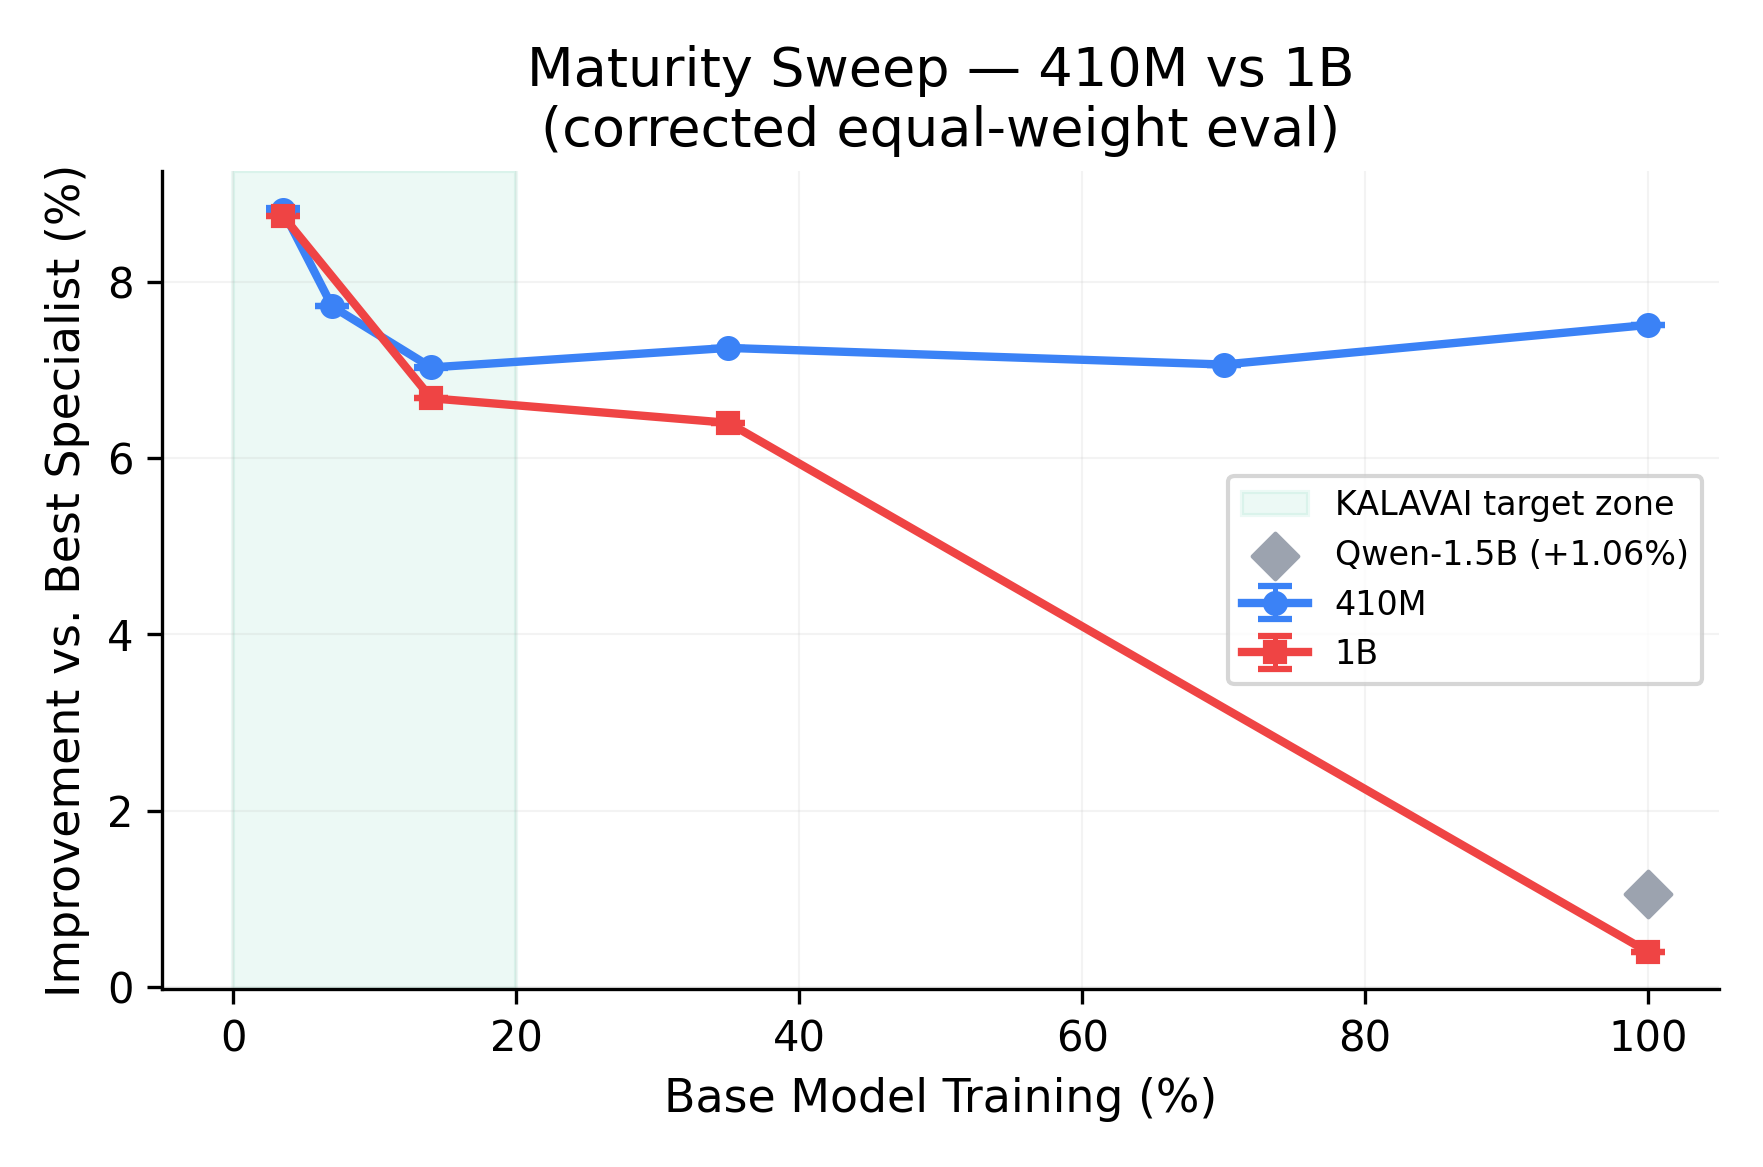
\includegraphics[width=0.85\textwidth]{fig_maturity_curve_combined}
  \caption{Maturity sweep results for Pythia-410M, Pythia-1B, and Qwen-1.5B across training checkpoints. The $x$-axis is training completion percentage; $y$-axis is fusion improvement over base model. Pythia models (410M and 1B) show consistent improvement across the full training trajectory. Qwen-1.5B at full training shows $-$1.0\%, a boundary condition attributed to Qwen's larger pre-training corpus already covering the specialist domains.}
  \label{fig:maturity}
\end{figure}

\section{5-Domain Specialist Scaling}
\label{app:scaling}

\begin{table}[h]
\centering
\caption{Specialist count scaling at Pythia-410M. The 2-specialist result uses only code and fiction domains (narrower evaluation drives the higher score). 3--5 specialists all achieve $\approx$14.1\% with near-zero variance. Improvement vs.\ best individual specialist on mixed held-out evaluation. All results: 3 seeds.}
\label{tab:scaling}
\begin{tabular}{rcccl}
\toprule
\textbf{Specialists} & \textbf{Domains} & \textbf{Improvement} & \textbf{Std} & \textbf{Note} \\
\midrule
2 & Code, Fiction & +17.73\% & $\pm$0.028\% & Narrower eval \\
3 & Code, Science, Fiction & +14.15\% & $\pm$0.029\% & Main config \\
4 & Code, Science, Fiction, Math (GSM8K) & +14.14\% & $\pm$0.019\% & \\
5 & + Multilingual (Spanish Wikipedia) & +14.12\% & $\pm$0.060\% & \\
\bottomrule
\end{tabular}
\end{table}

Adding specialists beyond the initial 3 does not dilute the improvement: 3, 4, and 5 specialists all achieve approximately +14.1\% with near-zero variance across seeds. The 2-specialist result (+17.7\%) is inflated because the evaluation set only contains two domains, and the router can achieve near-perfect specialisation on a 2-way split. These results suggest the mechanism scales to more specialists without degradation.

\section{Training Dynamics}
\label{app:dynamics}

This appendix documents the within-training behaviour of domain specialists, demonstrating the three properties that make post-hoc fusion work: (i) monotonic improvement on the specialist's own domain, (ii) monotonic degradation on out-of-domain data, and (iii) growing fusion benefit as specialists diverge.

\paragraph{Within-domain improvement and cross-domain degradation.}
Figure~\ref{fig:trainingcurves} shows the held-out evaluation loss for each specialist on each domain throughout training at Pythia-410M. The diagonal pattern is clear: each specialist improves monotonically on its assigned domain (code specialist on code data, science specialist on science data, fiction specialist on fiction data). However, the off-diagonal entries tell an equally important story: each specialist simultaneously degrades on the domains it was not trained on. By step 2,000, the code specialist evaluates at 2.908 on science data, worse than the base model's 2.892; the science specialist evaluates at 3.061 on fiction, worse than base (2.974). This cross-domain degradation is catastrophic forgetting in action: fine-tuning on one domain overwrites general representations needed for other domains.

This degradation is precisely why single-specialist dispatch fails catastrophically (Section~\ref{sec:failure}). Even with 99.3\%-accurate domain classification, a specialist assigned to an out-of-domain token will produce higher loss than the original base model, because the specialist has partially overwritten its cross-domain representations. The only way to recover is to run all specialists simultaneously and combine their outputs.

\paragraph{Growing fusion benefit.}
Figure~\ref{fig:fusiontrajectory} shows how the fusion benefit (MoE improvement over best individual specialist) evolves over specialist training steps. Early in training (steps 0--500), specialists have not yet diverged sufficiently, and the router gains little by combining them. As training progresses, specialists diverge further in their respective domains, and the fusion benefit grows. This trajectory has important implications for the training duration crossover (Section~\ref{sec:crossover}): the benefit peaks when specialists have diverged enough to be complementary but not so much that they can no longer be coherently combined. Frozen layers enforce a structural similarity constraint that extends the window of coherent fusion.

\paragraph{Cross-domain evaluation at training checkpoint.}
Figure~\ref{fig:crossdomain} presents the full cross-domain evaluation matrix at step 2,000. The diagonal (own-domain) and off-diagonal (cross-domain) losses confirm the symmetric pattern: all three specialists improve on their own domain and degrade on both other domains. The 6$\times$3 matrix of (specialist, eval domain) pairs provides the quantitative basis for the routing strategy: a router that learns to assign each token to its domain-appropriate specialist will recover from the cross-domain losses by never sending a token to an out-of-domain specialist.

\begin{figure}[h]
  \centering
  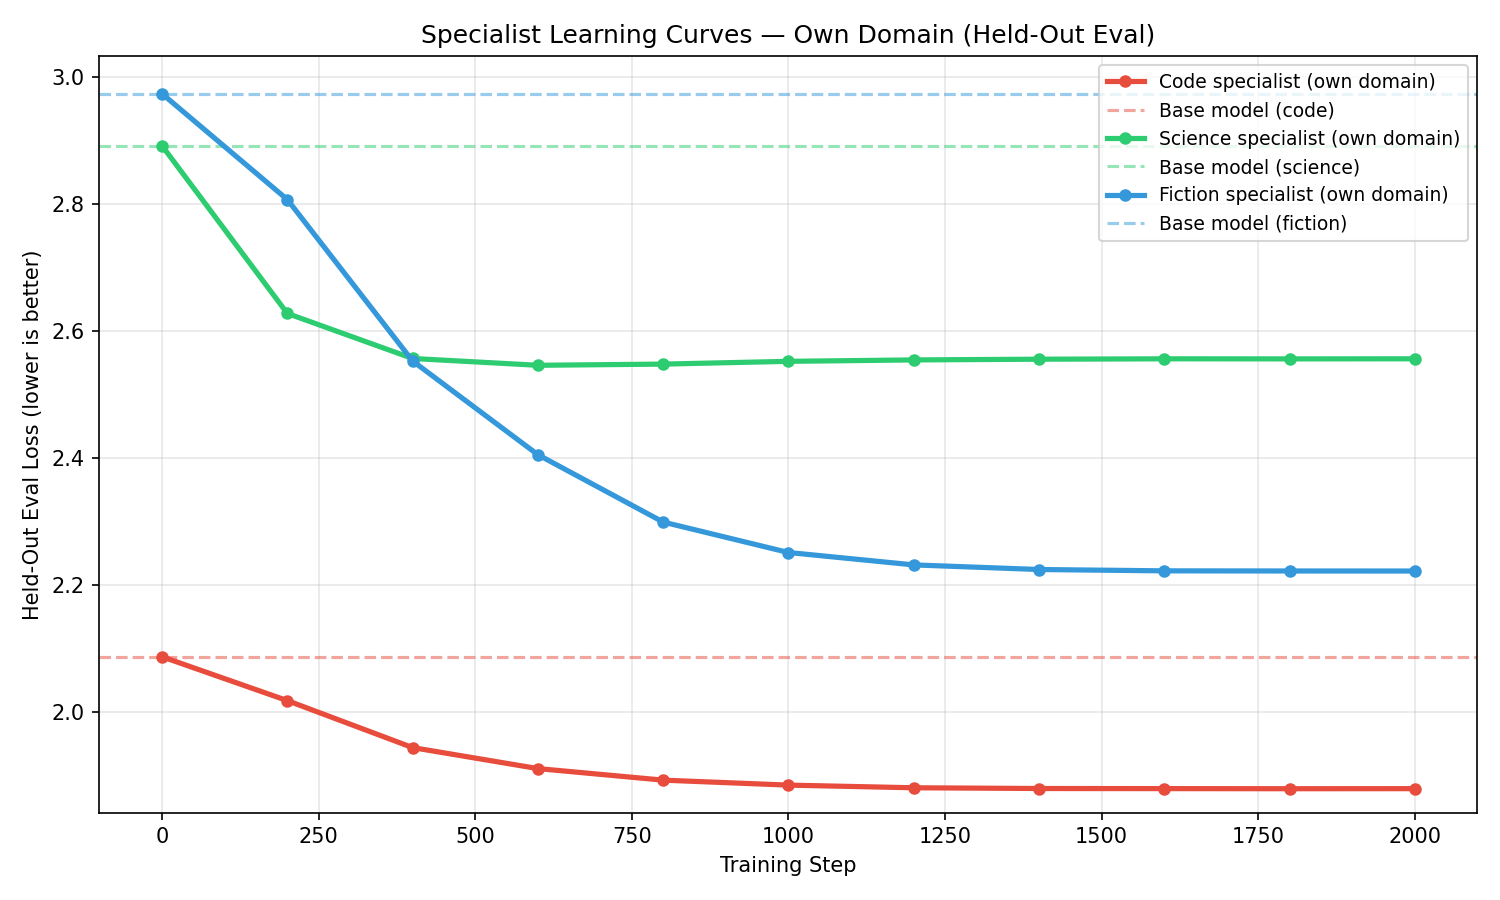
\includegraphics[width=0.85\textwidth]{fig_specialist_own_domain}
  \caption{Per-domain held-out evaluation loss for each specialist over training steps (Pythia-410M, freeze=4, seed=42). Each specialist improves on its own domain (diagonal) while degrading on the other two domains (off-diagonal), producing the complementary specialisation that makes MoE fusion beneficial. Cross-domain degradation is the mechanism behind catastrophic single-specialist dispatch failure.}
  \label{fig:trainingcurves}
\end{figure}

\begin{figure}[h]
  \centering
  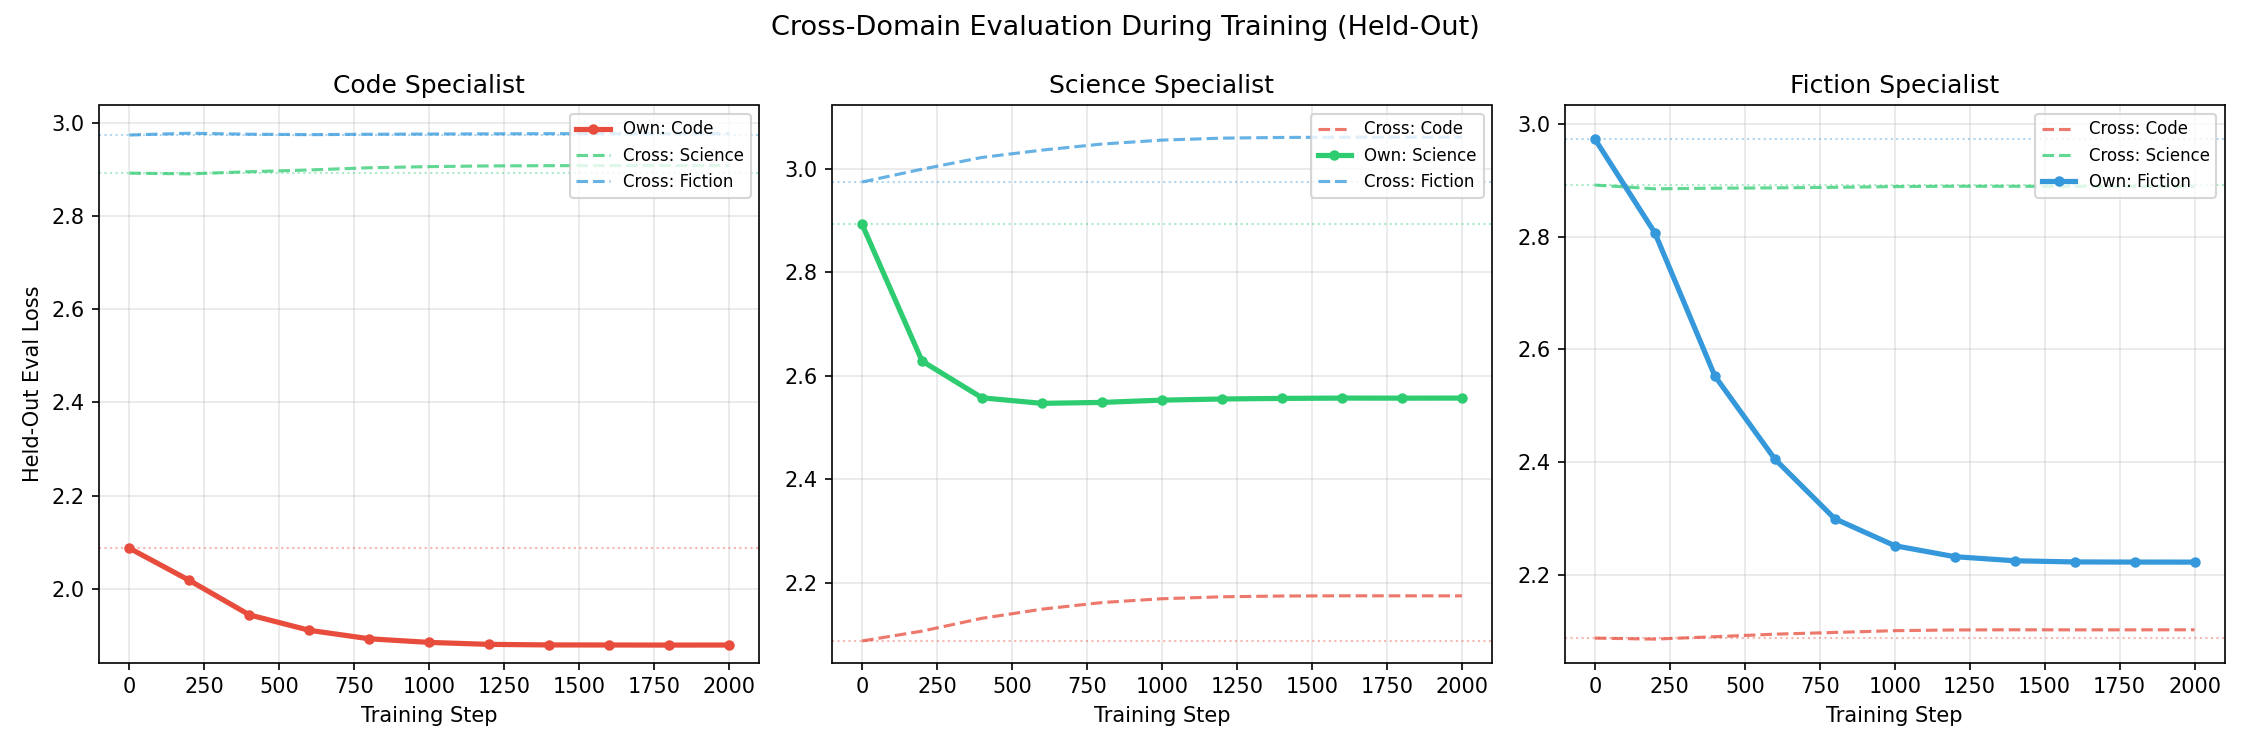
\includegraphics[width=0.80\textwidth]{fig_specialist_cross_domain}
  \caption{Cross-domain evaluation matrix at Pythia-410M step 2,000 (freeze=4, seed=42). Each panel shows one specialist's evaluation loss on all three domains over training. Dashed horizontal lines mark the base model's loss on each domain. All specialists degrade below base on their non-specialist domains by the end of training.}
  \label{fig:crossdomain}
\end{figure}

\begin{figure}[h]
  \centering
  
\includegraphics[width=0.75\textwidth]{fig_fusion_trajectory}
  \caption{Fusion benefit (MoE improvement over best individual specialist, \%) as a function of specialist training steps at Pythia-410M. Benefit grows monotonically up to approximately 5,000 steps, then plateaus (freeze=4) or degrades (freeze=0) at longer horizons. The crossover between freeze=0 and freeze=4 regimes is shown in Section~\ref{sec:crossover}.}
  \label{fig:fusiontrajectory}
\end{figure}

\section{Downstream Benchmark Results}
\label{app:benchmarks}

\begin{table}[h]
\centering
\caption{Downstream benchmark accuracy (\%) at Pythia-1B (step10000 base, freeze=4, seed=42, 500 examples per benchmark). Random chance: HellaSwag 25\%, ARC-Easy 25\%, LAMBADA 0\%, SciQ 25\%, WinoGrande 50\%.}
\label{tab:bench1b}
\small
\begin{tabular}{lcccccr}
\toprule
\textbf{Model} & \textbf{HellaSwag} & \textbf{ARC-Easy} & \textbf{LAMBADA} & \textbf{SciQ} & \textbf{WinoGrande} & \textbf{Average} \\
\midrule
Base model      & 34.4 & 40.4 & 60.2 & 68.4 & 49.6 & 50.6 \\
Code specialist & 34.2 & 39.4 & 57.4 & 65.8 & 50.0 & 49.4 \\
Sci. specialist & 34.2 & 41.0 & 56.4 & 65.8 & 48.2 & 49.1 \\
Fict. specialist & 34.4 & 39.8 & 58.6 & 66.8 & 48.2 & 49.6 \\
Weight average  & 34.6 & 39.0 & 57.8 & 67.8 & 48.6 & 49.6 \\
Monolithic      & 33.4 & 38.4 & 58.2 & 67.0 & 49.4 & 49.3 \\
\kalavai MoE    & \textbf{35.0} & 40.0 & 59.0 & 64.8 & 49.4 & \textbf{49.6} \\
\bottomrule
\end{tabular}
\end{table}

\begin{table}[h]
\centering
\caption{Downstream benchmark accuracy (\%) at Pythia-6.9B (step10000 base, freeze=6, seed=42, 500 examples per benchmark). Due to compute constraints at 6.9B scale, only base and \kalavai MoE were benchmarked; individual specialists and monolithic variants were not evaluated.}
\label{tab:bench6b}
\small
\begin{tabular}{lcccccr}
\toprule
\textbf{Model} & \textbf{HellaSwag} & \textbf{ARC-Easy} & \textbf{LAMBADA} & \textbf{SciQ} & \textbf{WinoGrande} & \textbf{Average} \\
\midrule
Base model   & 35.4 & 43.6 & 61.2 & 66.8 & 51.0 & 51.6 \\
\kalavai MoE & \textbf{35.6} & \textbf{45.2} & \textbf{62.8} & \textbf{67.8} & 49.4 & \textbf{52.2} \\
\bottomrule
\end{tabular}
\end{table}

At 1B scale, the MoE model leads on HellaSwag (35.0\% vs.\ 34.4\% base), the benchmark most sensitive to language modelling quality. Monolithic training produces the worst average accuracy (49.3\%), below even individual specialists (49.1--49.6\%), suggesting mixed-domain gradient interference degrades general reasoning as well as language modelling. At 6.9B, the MoE leads on four of five benchmarks, with an average improvement of +0.56pp over base. Downstream improvements are modest at these scales; we expect larger differentiation at 13B and above.

\section{Qwen-1.5B Negative Result}
\label{app:qwen}

Experiments with Qwen-1.5B at step 143,000 (full training, code and fiction domains, freeze=4, 2,000 steps, 3 seeds) produce a mean fusion improvement of $-$1.0\% $\pm$ 0.0\%. This negative result is a boundary condition, not a contradiction of the mechanism.

The Qwen-1.5B model is trained on a substantially larger and more curated pre-training corpus than Pythia, which includes the target domains (code, fiction) in high-quality form. At full training, the base model has already internalised domain-specific representations that are difficult to materially improve with 2,000-step fine-tuning. We observe that even the individual specialists barely improve over base on held-out domain evaluation (less than 1\%), which means there is no specialist advantage for the router to leverage.

This suggests a practical consideration: the \kalavai mechanism requires that specialist training produce meaningfully diverged representations from the base. If the base model is already domain-saturated, cooperative training adds no signal. The Pythia maturity sweeps show that saturation is not a concern for Pythia models even at step 143,000 (+14--15\% improvement), indicating the issue is specific to Qwen's pre-training distribution.

\section{Hybrid Routing Visualisation}
\label{app:routing}

Table~\ref{tab:routing} shows token-level gate weights for five hybrid-domain prompts. The router switches experts mid-sequence on all five prompts, with 11 total switches across the prompt set (2.2 per prompt on average).

\begin{table}[h]
\centering
\caption{Token-level gate weights (softmax over 3 experts: code, science, fiction) for hybrid-domain prompts. Pythia-410M, freeze=4, seed=42. Dominant weight ($>$0.5) shown in bold. ``---'' indicates transition token.}
\label{tab:routing}
\small
\begin{tabular}{p{3.5cm}lcc}
\toprule
\textbf{Prompt} & \textbf{Token} & \textbf{Dominant Expert} & \textbf{Weight} \\
\midrule
\multirow{3}{*}{\parbox{3.5cm}{``Write Python code to simulate the plot of Romeo and Juliet''}}
  & ``Write''    & Fiction & 0.787 \\
  & ``Python''   & Fiction & 0.821 \\
  & ``simulate'' & Fiction & 0.929 \\
  & ``plot''     & Code    & 0.540 \\
  & ``Juliet''   & Fiction & 1.000 \\
\midrule
\multirow{3}{*}{\parbox{3.5cm}{``Derive the equation for protein folding using Python pandas''}}
  & ``Derive''   & Fiction & 0.703 \\
  & ``protein''  & Science & 0.959 \\
  & ``folding''  & Fiction & 0.962 \\
  & ``Python''   & Code    & 0.585 \\
  & ``pandas''   & Code    & 0.998 \\
\midrule
\multirow{3}{*}{\parbox{3.5cm}{``Use calculus to analyze character development in Hamlet''}}
  & ``Use''      & Fiction & 0.852 \\
  & ``analyze''  & Science & 0.920 \\
  & ``character'' & Science & 0.794 \\
  & ``Ham''      & Fiction & 1.000 \\
\bottomrule
\end{tabular}
\end{table}

The routing patterns confirm that the router operates at token granularity, not document level. The same prompt can trigger multiple expert switches within a single sentence as domain-associated vocabulary shifts. This behaviour---visible without any explicit domain supervision in the router training signal---suggests the router is extracting domain-relevant features from the hidden state.

\begin{figure}[h]
  \centering
  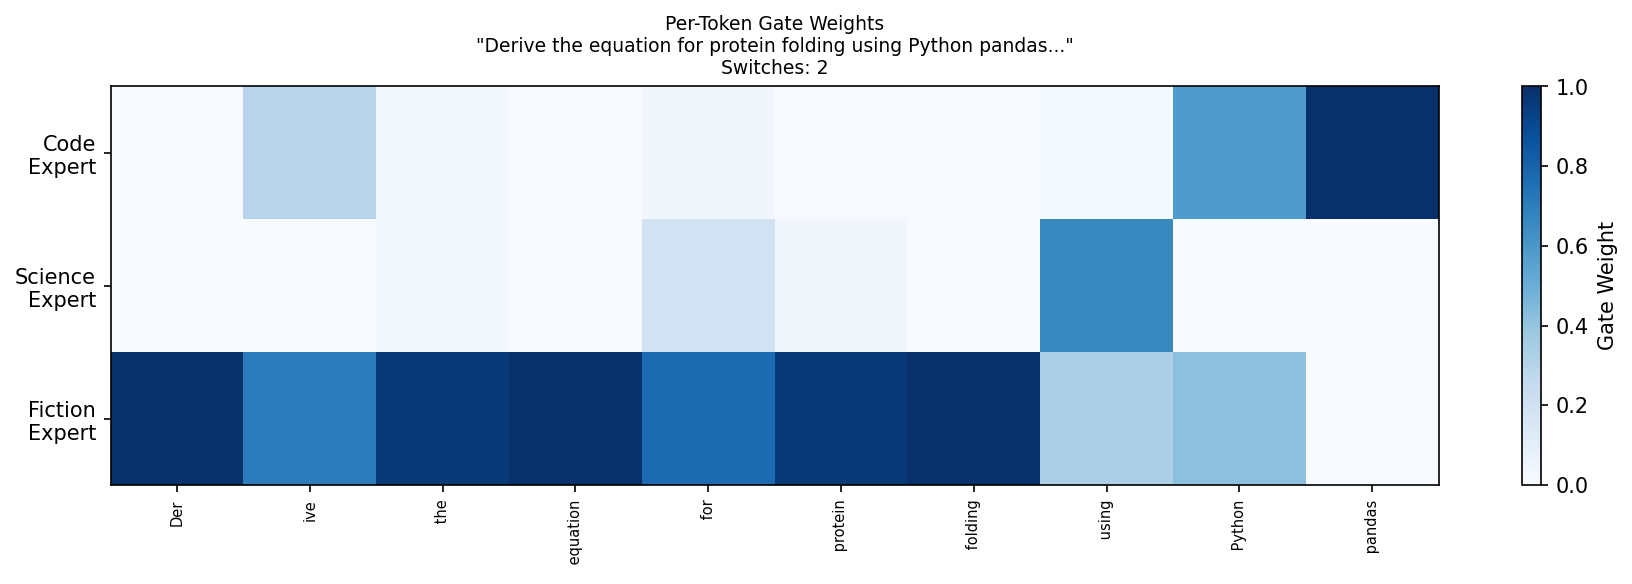
\includegraphics[width=0.9\textwidth]{fig_hybrid_routing_2}
  \caption{Gate weight heatmap for the prompt ``Derive the equation for protein folding using Python pandas'' (Pythia-410M, freeze=4, seed=42). Each column is a token; each row is an expert (code, science, fiction). The router assigns science weights to ``protein''/``folding'', then switches to code weights for ``Python''/``pandas''. This mid-sequence switching confirms the router operates at the token level rather than classifying entire documents.}
  \label{fig:hybridrouting}
\end{figure}

\section{Results Integrity Audit}
\label{app:audit}

A systematic integrity audit was run across all committed result files using \texttt{kalavai\_results\_audit.py}. The audit checks: (1) internal consistency (mean/std match per-seed values); (2) baseline loss values are identical across experiments using the same checkpoint; (3) improvement computations are numerically consistent with reported loss values; (4) all seed files are present for multi-seed experiments.

\textbf{Outcome: 322/322 checks passed, 0 issues detected.} Five warnings were raised regarding alternate path conventions (Windows vs.\ Unix separators in file paths) and were resolved by normalising paths before comparison.

The 6.9B \texttt{summary.json} file was not regenerated after the seeded evaluation fix and reflects stale pre-fix values (mean +2.72\%, std $\pm$8.17\%). All results in this paper use the corrected per-seed files (\texttt{step6\_fusion\_seed42.json}, \texttt{step6\_fusion\_seed137.json}, \texttt{step6\_fusion\_seed2026.json}), each of which reports +2.43\%--+2.44\%.

\end{document}
